\subsection{Solution: $\Theta(n lg_3 n)$}

\subsubsection{Divide-and-conquer approach}

I used divide-and-conquer's approach to solve the problem. \\

If $T(n)$ is the running time of a problem with $n$, in this problem, the size of the collection (e.g array). As is defined on Cormen's book explain, the problem generate $a$ subproblems, where each of which is $1/b$ the size of the previous problem. The algorithm will take $T(n/b)$ to solve one of the subproblems of size n/b, so, it takes $aT(n/b)$ to solve $a$ of them. Futhermore, the algorithm use $D(n)$ time to divide the problem into subproblems and $C(n)$ time to combine the solutions to the subproblems into the solution to the original problem, we get the recurrence equation: \\

\begin{center}
    $T(n) = aT(n/b) + D(n) + C(n)$
\end{center}

The problem of split your collection in a 3-way, is explained using the chosen approach: \\

\textbf{Divide:} It define 2 "middles" based on the size of the collection to break in 3 parts. It will take constant time, this means that $D(n) = \Theta (1)$. \\

\textbf{Conquer:} It recursively solve 3 subproblems, each of the size $n/3$. Thus, $aT(n/b) = 3T(n/3)$. \\

\textbf{Combine:} If it assumes that a 3-way subroutine exists with $\Theta (n)$ runtime. Thus, $C(n) = \Theta (n)$. \\

So, we get the recurrence:

\begin{center}
    $T(n) = 3T(n/3) + \Theta (1) + \Theta (n)$
\end{center}

It could use the recurrence tree intuitive steps below to get the result of $T(n/3)$ run time. 

\subsubsection{Recurrence Tree}

The recurrence tree is showed below, splitting the collection in a 3-way.

The algorithm progressively expands the 3-way tree, it finish when it get a 1-size array, or 1 element.

% image
\begin{figure}[h]
    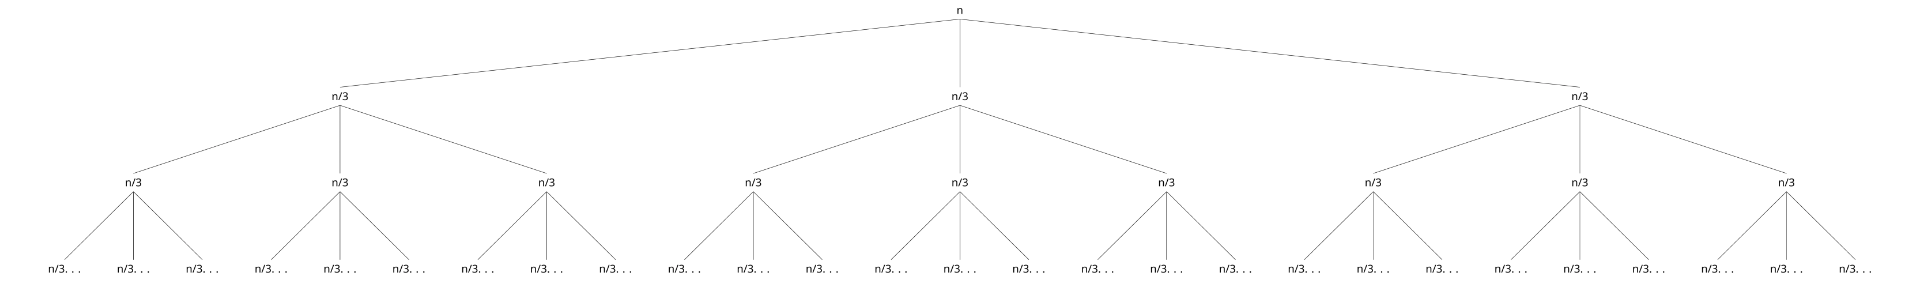
\includegraphics[scale=0.22]{sections/1warm_up/figures/tree.png}
    \caption{3-way tree}
    \centering
\end{figure}

This tree has $lg_3 + 1n$ levels. Then, it has a height of $lg_3 n$, where each level get a cost of n. Thus, the total cost is $n lg_3 n + n$, which means $\Theta(n lg_3 n)$.